% -*-coding: utf-8 -*-

\documentclass[compress,mathserif]{beamer}

\usepackage[utf8]{inputenc}
\usepackage[czech]{babel}
\usepackage[IL2]{fontenc}
\usepackage{amsmath}
\usepackage{amsthm}
\usepackage{amssymb}
\usepackage{amstext}
\usepackage{graphicx}
\usepackage{booktabs}
\usepackage{multirow}
\usepackage{dcolumn}

\newcolumntype{d}{D{,}{,}{4.2}}
\newcolumntype{k}{D{,}{,}{2}}
\newcolumntype{j}{D{,}{,}{1}}
\newcolumntype{u}{D{,}{,}{0}}

% Definice makra pro české uvozovky:
\def\bq{\mbox{\kern.1ex\protect\raisebox{-1.3ex}[0pt][0pt]{''}\kern-.1ex}}
\def\eq{\mbox{\kern-.1ex``\kern.1ex}}
\def\ifundefined#1{\expandafter\ifx\csname#1\endcsname\relax }%
\ifundefined{uv}%
        \gdef\uv#1{\bq #1\eq}
\fi

% beamer setup
\usetheme{Warsaw}
\beamertemplateballitem

\theoremstyle{definition}
\newtheorem{define}{Definice}

\theoremstyle{plain}
\newtheorem{thm}{Věta}

\newcommand{\beI}{\begin{itemize}}
\newcommand{\enI}{\end{itemize}}
\newcommand{\bL}{\mathbf{L}}


\title{Paralelní implementace fuzzy filtrů ve zpracování obrazu na GPU}
\author{Ladislav Horký}
\institute{FJFI ČVUT v Praze \newline \newline Vedoucí práce: Ing. Tomáš Oberhuber Ph.D.
\newline Konzultant: doc. Ing. Jaromír Kukal Ph.D.}
\date{\today}

\begin{document}
% úvodní slidy
	\begin{frame}
		\titlepage
	\end{frame}
	
	\section*{Obsah}   % nebude v obsahu
	\begin{frame}{Obsah}
		\tableofcontents
	\end{frame}

\section{Úvod}
    \begin{frame}{Cíle práce}
        \beI
            \item Seznámit se se základy fuzzy filtrů pro zpracování obrazu
            \item Seznámit se s programovacím prostředí CUDA
            \item Implementace vybraných algoritmů filtrace na CPU
            \item Provést paralelizaci algoritmů a implementaci na GPU
            \item Porovnat urychlení vůči CPU při použití různých datových typů
            \item Aplikovat algoritmy na reálná 3D obrazová data
        \enI
    \end{frame}

\section{Fuzzy Logika}

    \begin{frame}{Proč fuzzy?}
        Výhody
        \beI
            \item Solidní teoretický základ pro analýzu filtrů,
                postavený na \L ukasiewiczově algebře s odmocninou
            \item \alert<2>{Matematický model je přímo aplikovatelný na data,
                tak jak jsou reprezentována v počítači}
            \item Specializovaná na robustní odšumovací filtry
            \item Redukce na jednoduché matematické operace
            \item Možnost návrhu a analýzy sítí filtrů
        \enI
        Nevýhody
        \beI
            \item Několik oblíbených filtrů zde nelze implementovat (Gauss)
        \enI
    \end{frame}

     \begin{frame}{\L ukasiewiczova algebra s odmocninou}
        \begin{define}
            Nechť $\bL = [0,1]$ a $a,b \in \bL$. Nechť $\langle\bL,\wedge,\vee,\otimes,
            \rightarrow,0,1\rangle$, kde
            \begin{align}
                 a \wedge b &= \min(a,b) & a \otimes b &= \max(a+b-1,0)\notag\\
                 a \vee b &= \max(a,b) &  a \rightarrow b &= \min(1-a+b,1)\notag
            \end{align}
            je \textbf{reziduovaný svaz} s \textbf{\L ukasiewiczovou
            t-normou $\otimes$}, s největším prvkem 1 a nejmenším prvkem 0,
            pak $\langle\alert<2-4>{\bL,\wedge,\vee}\alert<3-4>{,\otimes,\rightarrow}\alert<4>{,sqrt},0,1\rangle$, kde
                 $$\mathrm{sqrt}(a) = (1+a)/2$$
            je \textbf{\L ukasiewiczova algebra s odmocninou}. Značíme ${\textit\L} A_{sqrt}$.
        \end{define}
    \end{frame}

    \subsection{Obraz ve fuzzy logice}
     \begin{frame}{Práce s 3D obrazem}
        \beI
            \item Pouze jednokanálové obrazy (odstíny šedi)
            \item \alert<2>{Hodnota výtupního voxelu je funkcí pouze voxelů ze sousedství
                (definovaného tzv. strukturním elementem) zdrojového voxelu}
            \item Tvar strukturního elementu má velký vliv na výsledek
            \item Z použití sousedství voxelu plynou problémy s okraji obrázku
        \enI
            \begin{figure}[h]
              \includegraphics[width = 0.8\textwidth]{img/masky.pdf}
              \caption{Tradiční strukturní elementy}
            \end{figure}
     \end{frame}


     \begin{frame}{Filtry}
        Roztřídění filtrů z implementačního hlediska:
        \beI
            \item Pomocné, algebraické (sčítání, prahování)
            \item Morfologické (eroze, dilatace, hrany)
            \item Odšumovací využívající seřazené pole (median, BES)
            \beI
                \item Založené na průměrování využívající Walshův seznam (H.L. median, WBES)
            \enI
        \enI
    \end{frame}

\section{GPU}

     \begin{frame}{Rozdíly CPU a GPU}
        \begin{figure}
            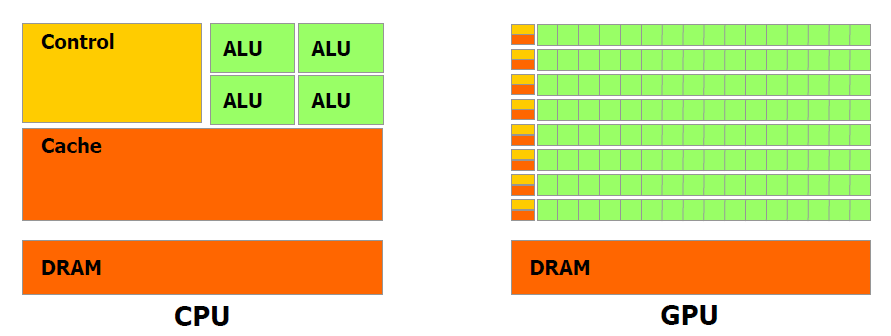
\includegraphics[width=90mm]{img/CPUGPU.PNG}
            \caption{Rozdíly v architektuře}
        \end{figure}
    \end{frame}

    \begin{frame}{Hlavní rozdíly v programování}

    \begin{minipage}{\textwidth}
        \begin{columns}
        \begin{column}{0.4\textwidth}
            \begin{center}
                CPU
            \end{center}
        \end{column}
        \begin{column}{0.6\textwidth}
            \begin{center}
                GPU
            \end{center}
        \end{column}
        \end{columns}
    \end{minipage}

    \begin{minipage}{\textwidth}
        \begin{columns}
        \begin{column}{0.4\textwidth}
            \begin{center}
                \beI
                    \item Velké odstupňované cache
                    \item Chytrý hardware
                \enI
            \end{center}
        \end{column}
        \begin{column}{0.6\textwidth}
            \begin{center}
                \beI
                    \item Hrubé odstupňování pamětí
                    \item Manuální, ale větší kontrola nad HW
                    \item Přísná pravidla pro přístup do paměti
                \enI
            \end{center}
        \end{column}
        \end{columns}
    \end{minipage}

    \begin{minipage}{\textwidth}
        \begin{columns}
        \begin{column}{0.4\textwidth}
            \begin{center}
                \beI
                    \item V případě více jader plnohodnotný MIMD
                    \item Cacheování instrukcí, branch-prediction
                \enI
            \end{center}
        \end{column}
        \begin{column}{0.6\textwidth}
            \begin{center}
                \beI
                    \item Pouze chytřejší, po částech vektorový procesor
                    \item Výpočet je paralelní, pouze pokud 32 současně běžících vláken vykonává stejný kód
                \enI
            \end{center}
        \end{column}
        \end{columns}
    \end{minipage}

    \end{frame}

\subsection{Implementace}
    \begin{frame}{Implementační postřehy pro GPU}
      Implementace na starší kartě 8800 GTX:
      \beI
        \item Překrývání latencí paměti - masivní paralelismus
        \item Šetření rychlou sdílenou pamětí
        \item Lepší je hloupější, ale nevětvící se program
        \item Využití manuální texturové cache
        \item U odšumovacích filtrů se problém redukoval na
            nalezení vhodného třídícího algoritmu
      \enI
    \end{frame}
\subsection{Algoritmy}
     \begin{frame}{Selekční algoritmy}
      Pro malá pole bylo GPU použito \textbf{Zapomnětlivé třídění}:
      \beI
        \item Spotřeba jen polovičního množství rychlé paměti, než je velikost tříděního pole (3/4 u BES)
        \item Větvení programu je minimální pro jakýkoliv vstup
        \item Lepší rozvrstvení přístupů do pomalé globální paměti pro vstupní data
        \item Náročnost $\mathcal{O}(n^2)$
      \enI
      Pro velká pole byl použit \bq hloupý\eq~$\mathcal{O}(n^2)$ algoritmus založený na
      zjištění počtu prvků větších a menších, než zkoumaný prvek.
      \vspace{5pt}
      
      Na CPU byl použit optimalizovaný \textbf{Introselect}.
    \end{frame}


\section{Výsledky}
    \begin{frame}{Testovací sestava}
        \begin{table}
        \begin{tabular}{lcc}
          \toprule
          & CPU & GPU \\
          \midrule
          \multirow{2}{*}{Název} & Intel & NVIDIA \\
          & Core 2 DUO & GeForce 8800 GTX \\
          Výpočetní & 2 & 128 \\
          jednotky & (využita 1) & (4 SM $\times$ 32 CUDA-jader) \\
          Frekvence & 1860 MHz & 1400 MHz \\
          Výpočetní & \multirow{2}{*}{---} & \multirow{2}{*}{1.0} \\
          schopnost & & \\
          Cache & 2 MB L2 & --- \\
          RAM/DRAM & 2 GB DDR2 & 768 MB GDDR3 \\
          FSB & 800 MHz & 1800 MHz \\
          \bottomrule
        \end{tabular}
        %\caption{Testovací sestava}
        \end{table}
        \begin{center}
           Testovací data: 3D SPECT obraz 79x95x69 voxelů
        \end{center}

    \end{frame}

    \begin{frame}{Urychlení morfologických filtrů}
        \begin{table}
        %\hspace{-0.1cm}
        \begin{tabular}{lkuku}
          \toprule
          Maska $\rightarrow$ & \multicolumn{2}{c}{kapacita masky: 26} & \multicolumn{2}{c}{kapacita masky: 18}\\
          Filtr $\downarrow$ & \multicolumn{1}{c}{GPU (ms)} & \multicolumn{1}{c}{Urychlení} & \multicolumn{1}{c}{GPU (ms)} & \multicolumn{1}{c}{Urychlení}\\
          \midrule
          \multicolumn{5}{c}{{\tt unsigned char} (0-255)}  \vspace{0.1cm} \\
          Eroze     & 1,47 & \textbf{30,2} & 1,34 & \textbf{24,0}\\
          Dilatace  & 1,47 & \textbf{30,3} & 1,37 & \textbf{23,8}\\
          Hrany     & 1,56 & \textbf{51,8} & 1,35 & \textbf{43,2}\\
          \midrule
          \multicolumn{5}{c}{{\tt unsigned int} (0-65535)}  \vspace{0.1cm} \\
          Eroze     & 1,61 & \textbf{31,0} & 1,37 & \textbf{26,9}\\
          Dilatace  & 1,62 & \textbf{30,9} & 1,37 & \textbf{27,1}\\
          Hrany     & 1,53 & \textbf{51,4} & 1,32 & \textbf{43,5}\\
          \bottomrule
        \end{tabular}
        %\caption{Srovnání morfologických filtrů na CPU a GPU pro různé datové typy}
        \end{table}
    \end{frame}

     \begin{frame}{Urychlení morfologických filtrů}
        \begin{table}
        %\hspace{-0.1cm}
        \begin{tabular}{lkuku}
          \toprule
          Maska $\rightarrow$ & \multicolumn{2}{c}{kapacita masky: 26} & \multicolumn{2}{c}{kapacita masky: 18}\\
          Filtr $\downarrow$ & \multicolumn{1}{c}{GPU (ms)} & \multicolumn{1}{c}{Urychlení} & \multicolumn{1}{c}{GPU (ms)} & \multicolumn{1}{c}{Urychlení}\\
          \midrule
           \multicolumn{5}{c}{{\tt unsigned char} (0-255)}  \vspace{0.1cm} \\
          Medián        & 9,45     & \textbf{33,9} & 3,62   & \textbf{58,3}\\
          BES           & 10,17    & \textbf{37,1} & 4,98   & \textbf{53,1}\\
          H-L Medián    & 735,76   & \textbf{4,3}  & 342,34 & \textbf{4,9} \\
          WBES          & 1124,46  & \textbf{4,2}  & 463,81 & \textbf{5,4} \\
          \midrule
          \multicolumn{5}{c}{{\tt unsigned int} (0-65535)}  \vspace{0.1cm} \\
          Medián        & 25,24    & \textbf{12,4} & 5,96   & \textbf{34,6} \\
          BES           & 10,95    & \textbf{35,6} & 6,45   & \textbf{42,5} \\
          H-L Medián    & 1327,99  & \textbf{2,3}  & 434,21 & \textbf{3,8}  \\
          WBES          & 1328,10  & \textbf{3,6}  & 520,38 & \textbf{4,9}  \\
          \bottomrule
        \end{tabular}
        %\caption{Srovnání morfologických filtrů na CPU a GPU pro různé datové typy}
        \end{table}
    \end{frame}

\subsection{Ukázky}
    \begin{frame}{Ukázky morfologických filtrů}

    \begin{columns}
    \begin{column}{0.3\textwidth}
        \begin{table}
          \begin{tabular}{ll}
            Originál \hfill & Hrany \hfill\\
            \vspace{2.5cm} & \\
            Eroze  & Dilatace \\
          \end{tabular}
        \end{table}
    \end{column}

    \begin{column}{0.6\textwidth}
    \begin{figure}
     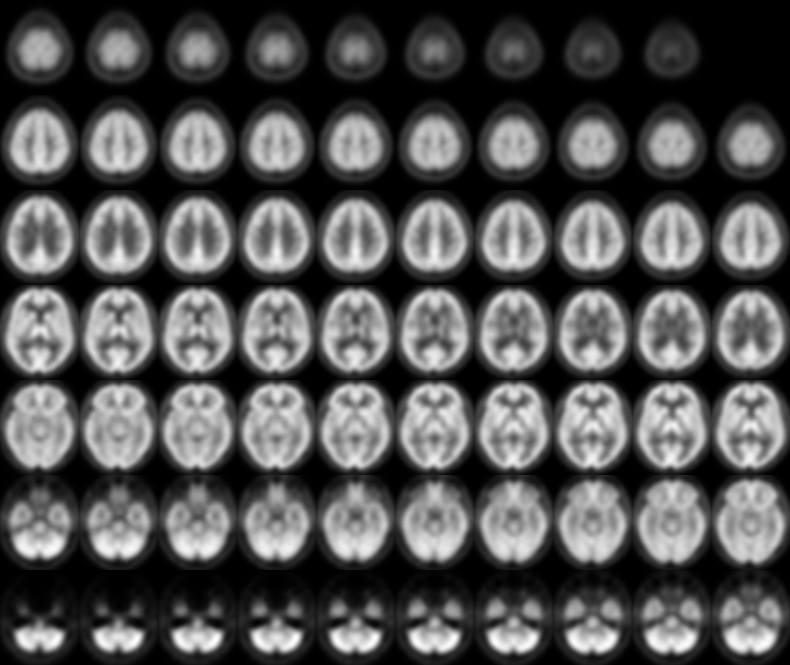
\includegraphics[width = 70pt]{img/original.png}
             \hspace{10pt}
     
\includegraphics[width = 70pt]{img/hrany.png}
    \end{figure}
    \vspace{-10pt}
    \begin{figure}
    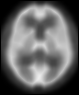
\includegraphics[width = 70pt]{img/eroze.png}
         \hspace{10pt}
    
\includegraphics[width = 70pt]{img/dilatace.png}
    \end{figure}
    \end{column}
    \end{columns}
    \end{frame}
    
    \begin{frame}{Ukázka BES}

    \begin{columns}
    \begin{column}{0.4\textwidth}
        \begin{table}
          \begin{tabular}{ll}
            \multirow{2}{*}{Originál} \hfill & kontaminace $5\%$ \hfill\\
            & šum $\sigma = 5/256$ \\
            \vspace{2cm} & \\
            Výsledek & Rozdíl od \\
            BES & originálu\\
          \end{tabular}
        \end{table}
    \end{column}

    \begin{column}{0.6\textwidth}
    \begin{figure}
     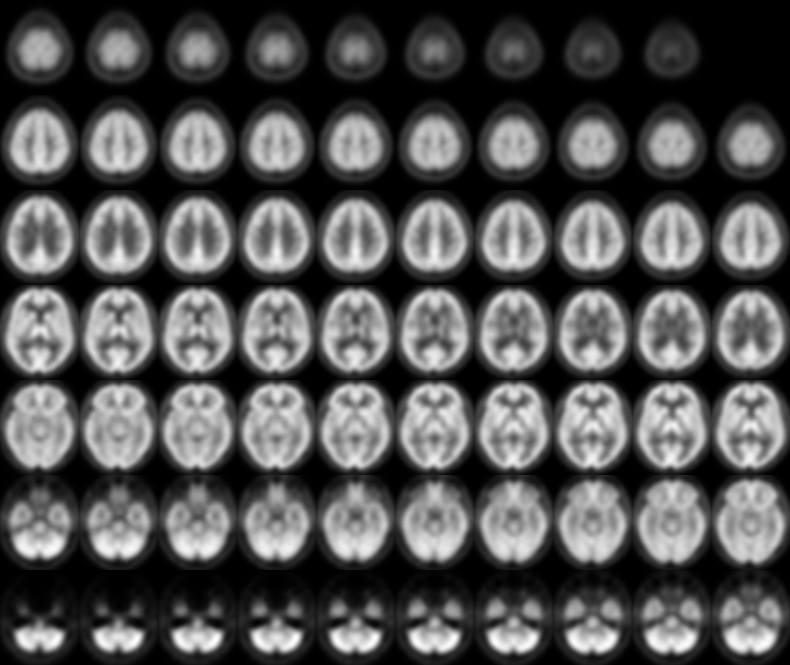
\includegraphics[width = 70pt]{img/original.png}
             \hspace{10pt}
     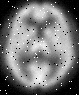
\includegraphics[width = 70pt]{img/5-30contaminated.png}
    \end{figure}
    \vspace{-10pt}
    \begin{figure}
    
\includegraphics[width = 70pt]{img/5-30bes.png}
         \hspace{10pt}
    
\includegraphics[width = 70pt]{img/5-30besD.png}
    \end{figure}
    \end{column}
    \end{columns}
    \end{frame}

\section{Závěr}
    \begin{frame}{Závěr}
      \beI
        \item Fuzzy logika se pro popis filtrů výborně osvědčila
        \item Některé filtry se podařilo zrychlit na jednotky ms, což je předpoklad pro použití v reálném čase
        \item Třídění (selekce) malých polí jako zajímavý problém pro GPU
        \item Lze odhadovat, kterým směrem se bude ubírat vývoj GPU
      \enI
    \end{frame}

    \begin{frame}{Dotaz oponenta I}
      Jakého zrychlení by bylo možné dosáhnout paralelizací na vícejádrovém CPU oproti sériovému výpočtu na CPU?

      \textbf{Odpověď:} Až maximální teoretická hranice -- n-násobek při použití n jader.
    \end{frame}


\end{document} 